
%%%%%%%%%%%%%%%%%%%%%%% file typeinst.tex %%%%%%%%%%%%%%%%%%%%%%%%%
%
% This is the LaTeX source for the instructions to authors using
% the LaTeX document class 'llncs.cls' for contributions to
% the Lecture Notes in Computer Sciences series.
% http://www.springer.com/lncs Springer Heidelberg 2006/05/04
%
% It may be used as a template for your own input - copy it
% to a new file with a new name and use it as the basis
% for your article.
%
% NB: the document class 'llncs' has its own and detailed documentation, see
% ftp://ftp.springer.de/data/pubftp/pub/tex/latex/llncs/latex2e/llncsdoc.pdf
%
%%%%%%%%%%%%%%%%%%%%%%%%%%%%%%%%%%%%%%%%%%%%%%%%%%%%%%%%%%%%%%%%%%%


\documentclass[runningheads,a4paper]{llncs}

\usepackage{amssymb}
\setcounter{tocdepth}{3}
\usepackage{graphicx}
%\usepackage{multicol}
\usepackage{epstopdf}	
\usepackage{fancyvrb}
					% incluye eps, 1ro los pasa a PDF y luego lo incluye

\usepackage{url}
\urldef{\mailsa}\path|{jcaccav, spedre, pdecris, akatz, dbenders}@dc.uba.ar|
\newcommand{\keywords}[1]{\par\addvspace\baselineskip
\noindent\keywordname\enspace\ignorespaces#1}

\begin{document}

\hyphenation{re-latively}
\mainmatter  % start of an individual contribution

% first the title is needed
\title{\LARGE{A new programming interface for Educational Robotics}}

% a short form should be given in case it is too long for the running head
\titlerunning{Programming for Educational Robotics}

% the name(s) of the author(s) follow(s) next
%
% NB: Chinese authors should write their first names(s) in front of
% their surnames. This ensures that the names appear correctly in
% the running heads and the author index.
%
\author{Javier Caccavelli \and Sol Pedre\and Pablo de Crist\'oforis \and Andrea Katz \and Diego Bendersky}
%
\authorrunning{Programming for Educational Robotics}
% (feature abused for this document to repeat the title also on left hand pages)

% the affiliations are given next; don't give your e-mail address
% unless you accept that it will be published
\institute{Departamento de Computaci\'on,\\
Facultad de Ciencias Exactas y Naturales, \\
Universidad de Buenos Aires \\
Buenos Aires, Argentina\\
\mailsa}

%
% NB: a more complex sample for affiliations and the mapping to the
% corresponding authors can be found in the file "llncs.dem"
% (search for the string "\mainmatter" where a contribution starts).
% "llncs.dem" accompanies the document class "llncs.cls".
%

\maketitle


\begin{abstract}
%Educational Robotics uses robotics as a teaching tool in middle and high schools, and undergraduate curricula. %and popularization of science. The goal is to use robotics for teaching a variety of subjects other than specifically robotics. To achieve this goal is vital to have an adequate interface that allows unexperienced students to interact with robots in an easy manner. In this paper we present the current development of ERBPI (\emph{Easy Robot Behaviour Programmign Interface}), a new application that doesn't require any previous programming experience to control robots. To accomplish this, we propose to abandon the imperative programming paradigm and take a behaviour-based approach. Thus, the new application is based on the connectionist paradigm. The idea is to program the behaviors of robots by establishing connections between its sensors and actuators. This connections may include different mathematical functions, making it possible to achieve complex behaviours. Moreover, different defined behaviours can be connected using a subsumission architecture. The new application is designed to work with a variety of real robots and simulators, and it is designed so that adding new robots and simulators is easy. Learning experiences with high school students allowed us to test its effectiveness.

Educational Robotics uses robots as a tool for teaching a variety of subjects other than specifically robotics in undergraduate curricula. %middle and high schools.  
To achieve this goal is vital to have an adequate interface that allows inexperienced students to interact with robots in an easy manner. In this paper we present the current development of ERBPI (\emph{Easy Robot Behaviour Programming Interface}), a new application that doesn't require any previous programming experience to control robots. To accomplish this, we propose to abandon the imperative programming paradigm and take a behaviour-based approach. Thus, the new application is based on the connectionist paradigm, accomplishing behaviours by establishing configurable connections between sensors and actuators. Moreover, different defined behaviours can be connected using a subsumption architecture. The new application is designed to work with different robots and simulators, and it is simple for adding new ones. Learning experiences with high school students allowed us to test its effectiveness.

%comentario sol: me parece que hablar de paradigma conexionista es demasiado... mas bien creo q no existe. 
\keywords{educational robotics, behaviour-based programming interface.}
\end{abstract}


\section{Introduction}
\label{sec:intro}

The use of robots in undergraduate curricula has grown over the last years. The availability of low cost, easy-to-use platforms has even led to the use of robots in middle and high schools. Many teachers have an interest in introducing robots into their classrooms for teaching a variety of subjects other than specifically robotics. Thus, Educational Robotics arises, proposing the use of robotics as a teaching resource that allows inexperienced students to approach different scientific fields such as mathematics, experimental sciences, technology, information science and computing, among others. One of the aims of Educational Robotics is to aid students in building their own representations and concepts of science and technology, through the use, handling and control of robotic environments. This approach uses the constructionist process of designing, building, programming and debugging robot's behaviours, as well as collaboration and teamwork, as powerful means of enlivening education. 
%***citas del paper de Aibo [2, 6, 7]**** ver bien el afano de citas en este parrafo del primer parrafo de ambos papers.

Several educational robotics programming interfaces have been presented. Most are designed for university-level or late high school students and are implemented as extensions to existing programming languages. That is the case of Pyro \cite{pyro}, a Python-based programming framework which provides a set of abstractions that allow students to write platform-independent robot programs. Other interfaces include Not-Quite C (NQC) \cite{nqc} based on C, BrickOS \cite{brickos} based on C++ and leJOS \cite{lejos} that is based on Java. These three interfaces are particular for Lego Mindstrom. All these interfaces require programming experience or interest in learning a particular programming language. This makes them unsuitable for middle or high school students that do not handle any imperative or procedural programming concepts, such as the idea of loops, conditions, forks or variables in a program. %Educational Robotics courses, which aim at teaching subjects other than robotics or programming. 
Microsoft also offers the commercial tool Microsoft Robotics Developer Studio \cite{mrds}. This includes a visual programming interface based on a data flow approach, but again it requires knowledge of programming concepts, making it quite complex for inexperienced users. 

There are also several graphical environments for simulated robots aimed at middle schools. That is the case of StartLogo \cite{startlogo}, Squeak Etoys \cite{etoys} and Scratch \cite{scratch}. These are easy-to-use programming interfaces, allowing inexperienced students to make a quick start, although they maintain an imperative programming influence and are designed only for particular simulated environments. Another programming interface used in instructional settings at the K-12 level is RoboLab \cite{robolab} for the LEGO Mindstorms robot. This is a graphical environment in which students are given palettes of icons that they can drag and drop on a canvas. The icons represent robot components like motors and sensors, as well as abstract programming structures such as loops and counter variables. This interface is particular for the Mindstrom robot, and once again uses imperative programming structures that add complexity to the robotic environment. Finally, in \cite{robolab-ext} authors present an extension to RoboLab in order to work with other robotic platforms. 

%There are many works describing programming interfaces for Educational Robotics ***citas papers que presenten interfaces ***. Many of them emphasize the proposed applications as didactic tools, easy to learn and use for unexperienced public. To our knowledge, all involve the use of the imperative paradigm in some way for programming robots, . It is not clear if these applications are really easy to use for users that do not handle any imperative or procedural programming concepts, such as the idea of cycles, conditions or forks in a program.

Our experiences working with classroom teachers and young students have raised several issues that have motivated us to pursue the development of a behaviour-based interface, which abstracts away the imperative programming constructs and the low-level motor and sensor commands that often confuse inexperienced programmers or deter techno-phobic students. To accomplish this, we propose to abandon the imperative programming paradigm and take a behaviour-based approach. Thus, the proposed interface is based on a connectionist paradigm. The idea is that stimuli captured by the robot sensors are processed in a network of connections and result in a response for the robot actuators. To program the robot behaviours we have to establish connections between its sensors and actuators. This connections may include different mathematical functions \cite{braitenberg}. Moreover, different defined behaviours can be connected using a subsumption architecture \cite{subsumicion}, making it possible to achieve more complex behaviours. In this way, we get a state automaton (or machine), where each state represents a behaviour and each transition a change in the environment. This state machine can be easily translated into an imperative program that the robot executes to perform the behaviour.

This paper describes the current development of ERBPI(\emph{Easy Robot Behaviour Programming Interface}), a behaviour-based, easy to use robotic programming interface for Educational Robotics that allows to program different robotic platforms and simulators. The design of ERBPI follows the next criteria:

\begin{itemize}
\item \emph{Ease of use:} The user is not supposed to have any previous programming knowledge. The interface must be intuitive and easy to learn, providing all the tools to program robot behaviours graphically, making it possible to perform drag-and-drop with robot's sensors and actuators, build sensor-actuator connections, and easily configure them. 

\item \emph{Platform independence:} The application must work with a variety of robots and simulators, and be easily expandable to control new ones. The different bodies, sensors, actuators, low-level commands and protocols to communicate with high-level systems of different robots must be abstracted. Moreover, users must be able to test and run the same behaviours on multiple robots.

%\item \emph{Expressive power:} The application has to have a computing capacity similar to that provided by programming languages based on the imperative paradigm. This is necessary to perform complex robot behaviours. Our application use a connectionist paradigm to buid basic behaviours and subsumition architecture to build an automaton of state to interconnect them, making possible to achieve more complex behaviours. %(Comentario de Pablo: hasta que no tengamos una demostración formal de que lo que creamos es Turing Compatible no podemos afirmar que tenemos un poder de expresividad equivalente a los programas imperativos. Por eso puse la palabra "similar". Para mi, si en algún momento hacemos esta demostración tenemos un paper para una revista!)
%\item \emph{Comprehensive expressive power:} VER Q PONER ACA - FALTA

%\item \emph{Good for testing and debbuging environment:} PONEMOS ALGO DE LA IDEA DEL DEBUG Y TESTING CON LA WEBCAM? - FALTA (Comentario de Pablo: El problema es que no sabemos si esto realmente se va a poder hacer y no tenemos nada hecho de esto. Yo de la cámara no pondría nada).

\item \emph{Portability:} The application must work in different operating systems and platforms to accommodate the different hardware and software available in schools or other educational institutions.  

\item \emph{Flexibility:} Students from a wide range of backgrounds and teachers with a broad range of goals must be able to use the programming interface effectively, accommodating different levels, curricular needs, academic subjects and physical environments for instruction.

\end{itemize}

This paper is organized as follows. In the next section we describe ERPBI's architecture and features, and give examples of use. Afterward, we comment some experiences using ERPBI in the classroom with high school students. Finally, we draw some conclusions and discuss directions for future work.


\section{The ERBPI: Easy Robot Behaviour Programming Interface}
\label{sec:erbpi}

%\begin{itemize}
%\item mini seccion que repita idea
%\item seccion que describe la arquitectura y cada modulo.
%\item aspectos de implementacion (resumidos) 
%\item seccion que muestra un ejemplo de programación.
%\end{itemize}

%En esta secci\'on describiremos la arquitectura de la interfaz ERBPI. 
%Para el dise\~no de la misma, hemos decidido optar por un dise\~no modular que brinde responsabilidades claras y delimitadas en los m\'odulos, donde una modificaci\'on en un m\'odulo impacte lo menos posible en el resto de la aplicaci\'on, y que al mismo tiempo nos brinde tambi\'en la posibilidad de extensibilidad de caracter\'isticas de la aplicaci\'on, dandole  la capacidad de adaptarse a los cambios de requerimientos, pudiendo ser extendida con facilidad, sin la necesidad de sufrir modificaciones. Hasta este momento hemos implementado los distintos m\'odulos que componen la aplicaci\'on y que detallaremos m\'as adelante: CORE, RAL y GUI. Nos queda pendiente aun realizar la implementaci\'on del feature de subsumici\'on.
 

%Como dijimos anteriormente, la interfaz de programaci\'on de robots ERBPI utiliza el paradigma conexionista para programar los comportamientos del robot. La aplicaci\'on permite al usuario establecer conexiones entre los distintos sensores y actuadores del robot. Cada conexi\'on puede ejecutar una funci\'on matem\'atica dando lugar a un grafo de ejecuci\'on that perform the basic behaviour (Fig. \ref{Fig:grafo})

ERBPI uses a behaviour-based approach following the connectionist paradigm. It enables users to create basic behaviours, and then connect them using a subsumption architecture to create more complex ones. 

To create basic behaviours, the user establishes connections between sensors and actuators, and configures them with a chain of mathematical functions.  Each function can have several inputs, including sensed data and outputs from previous ones. It uses all the inputs to compute a single output, that in turn may be used to set actuators or input following functions. The user chooses functions from predefined families and configure their parameters. %This output may be used to set one or more actuators, or to input a following function. 
This schema defines an execution graph that allows to infer a computation order and thus translate it to an imperative program for the robot. 

%\begin{figure}
% \centering
% 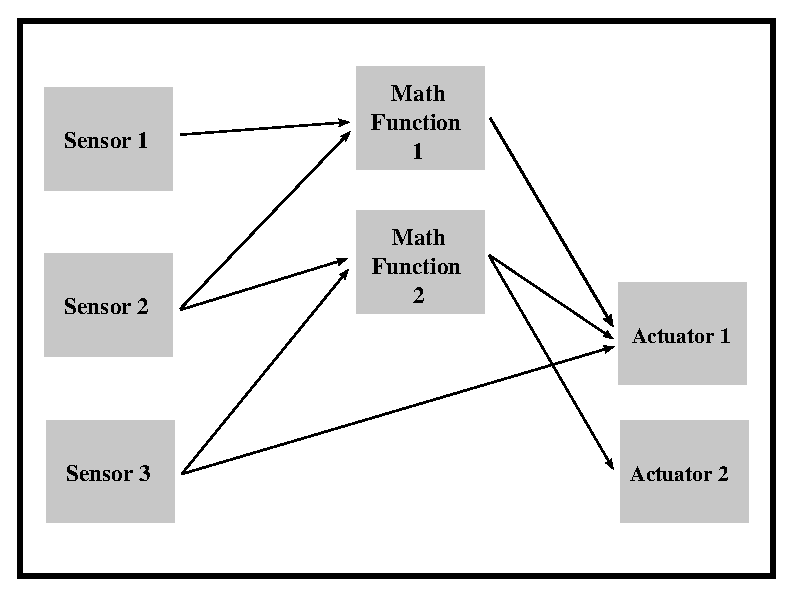
\includegraphics[scale=0.5]{images/grafo_eng.eps}
% \caption{An example of execution graph.}
% \label{Fig:grafo}
%\end{figure}

All the function outputs, sensors and actuators values are normalized to the same scale ($-100, 100$). This scale is a ``percentage of activation'' for each element in the schema. Normalizing all the data permits the previous schema to work properly and also that one behaviour can be used for several robots that may have different sensors or actuators. %The translation of this normalized values to actual sensors or actuators values is performed by a particular robot abstraction layer, explained in section \ref{sec:RAL}.

%Different basic behaviours can be connected using a subsumision architecture, making it possible to achieve more complex behaviours. In this way, we get a state automaton, where each state represents a behaviour and each transition a change in the environment. This state machine can be easily translated into an imperative program that the robot executes to perform the behaviour.

The application has a modular design, clearly decoupling the different responsibilities in the system. The GUI (Graphical User Interface) module allows the user to graphically design the robot behaviour, and then exports this behaviour in a file. The CORE module reads this file and executes the defined behaviour. To communicate with the robotic platform (simulator or real robot), the CORE uses a particular RAL (Robot Abstraction Layer) module. There is one RAL for each robotic platform ERBPI manages. This module is in charge of normalizing all the sensor and actuator values, and also of communicating with the actual robot using its particular communication protocol. The basic architecture, including the three modules and their communication, is shown in Fig. \ref{Fig:arquitectura}. Each module is explained in the following sections. 

%La idea general de esta arquitectura es que mediante el m\'odulo GUI el usuario pueda programar el comportamiento del robot de forma gr\'afica y sensilla. Una vez hecho esto, el comportamiento es entregado al m\'odulo CORE que se encarga de ejecutar el comportamiento, utilizando el módulo m\'odulo RAL, que ser\'a el encargado de establecer la conexi\'on entre el CORE y el robot correspondiente.

%Es importante tener en cuenta, como dijimos antes, que hemos dado a la aplicaci\'on la capacidad de poder ser extendida en muchas de sus caracter\'isticas sin la necesidad de ser modificada. Para esto, como veremos m\'as adelante, junto al dise\~no modular se utilizar\'an est\'andares de intercambio de informaci\'on, como XML (Extensible Markup Language), que permitir\'an tanto la comunicaci\'on entre los m\'odulos como la configuraci\'on de los mismos y de toda la aplicaci\'on, features setting, agregar robots, modificar caracter\'isticas de los robots, etc. 

%En la Fig. \ref{Fig:arquitectura} podemos ver la arquitectura de la aplicaci\'on, con sus tres m\'odulos y la comunicaci\'on entre ellos. A continuación vamos a explicar cada módulo en detalle.

\begin{figure}
 \centering
 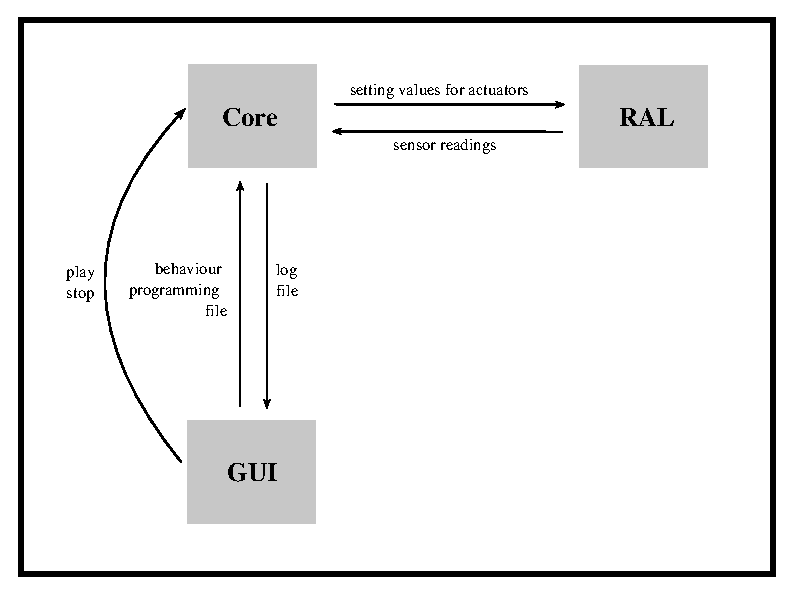
\includegraphics[scale=0.7]{images/arq_eng.eps}
 \caption{ERBPI's modular architecture.}
 \label{Fig:arquitectura}
\end{figure}

\subsection{GUI (Graphical User Interface) Module}

The GUI module is in charge of interacting with the user. To start, the user selects a robot or simulator to work with. The GUI enables the user to drag and drop elements (sensors, actuators, functions) to a work canvas, and then connect them using the mouse. Different functions may be selected from a menu, dragged to the canvas, and then configured with a pop-up configuration window. Fig. \ref{Fig:guiCanvas} shows a screenshot of the GUI and Fig. \ref{Fig:guiFunction} an example of the pop-up configuration window. 

%El módulo GUI (Graphical User Interface) se encarga de la interfaz con el usuario. Primero debemos seleccionar con qué robot (o silumador) queremos trabajar. Luego seleccionamos los sensores y actuadores del robot que vamos a usar para el comportamiento que queremos hacer. Mediante mecanismos muy sencillos de arrastrar y soltar (drag-and-drop) los diferentes objetos (sensores, actuadores, conexiones) en un escritorio de trabajo, podremos generar diferentes comportamientos. Cada conexión sensor-actuador posee una ventana emergente que permite definir funciones matemáticas parametrizables. De esta forma, el usuario construye un grafo de ejecución que representa el comportamiento a realizar, donde los nodos son los sensores, actuadores y funciones matemáticas, como podemos apreciar en la Fig. \ref{Fig:gui01} 

\begin{figure}
 \centering
 \includegraphics[scale=0.3]{images/gui_canvas.png}
 \caption{A screenshot of the application. The upper panel shows the configurations and elements. The general operations (new, open, save, play, quit) are in the upper left corner. The upper-center panel has different families of functions the user can choose from (decreasing, growing, broken and constant functions in this screenshot). The upper right panel shows the selected robot with its sensors. In the canvas we can see a line following behaviour that stops when the bumpers are activated.}
 \label{Fig:guiCanvas}
\end{figure}

\begin{figure}
 \centering
 \includegraphics[scale=0.3]{images/gui_function.png}
 \caption{The configuration pop-up window for a broken function. The change points in the function and the low and high levels can be easily configured moving them with the mouse. The scale for the normalized values ($-100, 100$) is also observable. }
 \label{Fig:guiFunction}
\end{figure}
%Otra caracter�stica importante del m�dulo GUI es que tiene la funci�n de ser la interfaz gr�fica de la aplicaci�n completa, coordinando el funcionamiento de los distintos m�dulos. De esta forma, 

Once the behaviour is finished, the user can select a robot to execute it on. The created behaviour and the minimal sensor and actuator configuration needed for its execution are stored in a file (the behaviour-file), that will be read by the CORE. The execution of the behaviour may be started and paused at any moment from the GUI. The GUI also provides general operations to open and save files. 

The GUI is implemented in Java, a good language for graphical interfaces and portable to several operating systems, only requiring the installation of the JVM (Java Virtul Machine). The behaviour-file is in XML(Extensible Markup Language), making it very simple to add new robots, sensor types, functions and other features we might add to ERBPI. A simple example of a behaviour-file is shown in table \ref{xml}. 


\begin{table}[ht!]
\footnotesize
\begin{Verbatim}[frame=single]
     <behaviour> 
       <sensors>
         <sensor id='sonar.0'/>
         <sensor id='encoder.motor.left'/>
       </sensors>
       <functions>
         <function id='function1'>
           <inputs>
             <input id='sonar.0'/>
             <input id='encoder.motor.left'/>
           </inputs>
           <points>
             <point x='100' y='0'/>
             <point x='150' y='255'/>
           </points>
         </function>
       </functions>
       <actuators>
         <actuator id='motor.left'>
           <inputs>
             <input id='function1'/>
             <input id='function2'/>
           </inputs>
         </actuator>
       </actuators>
     </behaviour>
\end{Verbatim}
\normalsize
\caption{Example of an XML behaviour-file. In this case, two sensors are needed to perform this behaviour (a sonar and an encoder). A broken function (\texttt{function1}), defined by two points, takes both sensors as inputs. The value for the motor.left actuator is set by the output of two functions}
\label{xml}
\end{table}

%En este caso hemos utilizado el lenguaje de programación Java para la implementacion. Hemos realizado esta elección por la capacidad de portabilidad de este lenguaje y la no necesidad de recompilar para distintos Sistemas Operativos.

%Una vez creado el comportamiento para el robot, podemos indicar sobre cuál robot se ejecutará. %y ejecutarlo con tan s�lo presionar \textit{play} en la GUI. 
%El comportamiento creado y la configuración de sensores y actuadores requerida para el robot en cuestión se guardan en un archivo de configuración que es entregado al múdulo CORE para su ejecución. La ejecución del comportamiento puede iniciarse y pausarse en cualquier momento también desde la GUI. Además la interface tiene botones para guardar el comportamiento en cuestión o abrir otro generado previamente.

\subsection{CORE module}

The CORE module is in charge of executing the behaviour. It reads the XML behaviour-file and establishes a connection with the appropriate RAL. At regular intervals, the core receives from the RAL the normalized values of the sensors, executes the behaviour, and gives to the RAL the normalized values to set the actuators. The CORE stops when the GUI signals the user has stopped the execution. 

To be able to execute the behaviour, the CORE has to transform the execution graph defined by the GUI in the behaviour-file to a corresponding ordered execution list, to guarantee that all the inputs for a function are ready when its turn to execute is up. For this, we used a topological sorting \cite{topologicalSorting} of the execution graph. The CORE also asserts that the behaviour can be executed in the selected robot, for example that the graph is not cyclic (i.e, cannot be ordered) or that the robot has enough sensors and actuators to execute the behaviour. It also defines the communication frequency with the RAL depending on the robots working frequency. Finally, the CORE makes a log-file where all the values at a certain time are registered, including each sensor value, the output value of each function and the value of each actuator. This log file is communicated to the GUI. We plan to use it to implement a debug function in the future. 


%El modulo CORE es el encargado de leer el archivo de comportamiento y ejecutarlo. Para esto, debe establecer una conexión con el múdulo RAL (Robot Abstraction Layer), le envia comandos para los actuadores del robot y recibe del RAL el estado del robot. Otra tarea del CORE es realizar una serie de chequeos correspondientes a la factibilidad de ejecución de ese comportamiento en el robot indicado. Por ejemplo, si el comportamiento definido por el usuario da lugar un gráfo acíclico que puede ser ejecutado secuencialmente, o si el robot posee los sensores y actuadores requeridos para llevar a cabo ese comportamiento. El módulo CORE también debe definir la frecuencia con la que se comunica con el RAL, dado que cada robot o simulador tiene una frecuencia de trabajo diferente dependiendo de sus unidades de procesamiento, sensores y actuadores. 
%Por último, el CORE lleva un registro de todo lo sucedido a traves de un archivo de \textit{log}, donde se deja registo del valor de cada sensor, de la función matemática que aplica en la conexión sensor-actuador y del valor actuador a cada momento, y que comunica a la GUI para poder realizar \textit{debug} del comportamiento del robot.

\subsection{RAL (Robot Abstraction Layer) module}
\label{sec:RAL}

The RAL modules encapsulates all the knowledge of the particular robot or simulator, providing a standard interface to the CORE module, dealing with everything necessary to communicate with the actual robot. The RAL abstracts the particular robot, its communication protocol, and normalizes the values of the particular sensors and actuators. In this way, all the specific characteristics of the robot are transparent to the CORE. A RAL must implement a standard interface that include the following methods:  get the list of sensors and actuators in the robot, get the frequency the robot can work in, get the sensor values, and set the values for the actuators. To add a new robotic platform for ERBPI to work with, a developer must only program a particular RAL for the platform implementing the general RAL interface.

All RALs are implemented as dynamic libraries. In this manner, we can add new RALs without having to recompile the CORE or the GUI. Moreover, this allows the CORE to load a different RAL on runtime, without having to restart the application. This makes ERBPI easily extendable to control different robots.

To the date, we have implemented RALs for the Khepera \cite{khepera} and Exabot \cite{exabot} robots, and for the YAKS (Yet another Khepera Simulator) \cite{yaks} and the Player/Stage \cite{player} simulator. 

%Hasta el momento, hemos implementado los RALs de dos robots y dos simuladores de los que disponemos en nuestro laboratorio: Khepera robot, YAKS (Yet Another Khepera Simulator), ExaBot robot, Player/Stage simulator.

%El modulo RAL se encarga de la comunicacion entre el CORE y el robot (real o simulado). 
%Como la aplicacion está concebida para trabajar con una amplia gama de robots y simuladores, necesitamos una capa de abstraccion respecto del hardware específico donde se va a ejecutar el comportamiento, es decir, qué tipo de robot, qué cantidad y tipo de sensores y actuadores, que tipo de comunicacion se utilizada para la conexion con el robot, etc.
%Por lo tanto, la características específicas de cada robot son transparentes para el módulo CORE, que solo se comunicara con el RAL para obtener el estado del robot y enviar el nuevo valor para sus actuadores. Luego, sera el RAL el que se comunicara directamente con el robot (real o simulado) segun corresponda.

%El RAL contiene una serie de funciones para obtener la lista de sensores y el estado de los mismos, obtener la lista de actuadores y setear el estado de los mismos y obtener la frecuencia de trabajo del robot.

%Para agregar un nuevo robot para trabajar con la aplicacion, solo deberemos programar el nuevo RAL correspondiente de ese robot e indicarle a la GUI en su archivo de configuración la existencia del nuevo robot.

%\subsection{Implementation issues}

%ERBPI is an open source project, so we used all open source libraries. We also used standard programming languages that 
%Hemos decidido realizar el desarrollo de la aplicación siguiendo los lineamientos de Software Libre, dando la libertad a los usuarios de la aplicacion para ejecutar, copiar, distribuir, estudiar, cambiar y mejorar el software. Siguiendo el mismo enfoque, y como pretendemos la mayor portabilidad posible de la aplicación a distintos ambitos (talleres en escuelas, charlas y demostraciones en diferentes instituciones, etc), también elegimos lenguajes de programacion estandares que puedan ser compilados y ejecutados en los sistemas operativos mas comunes como Windows o Linux. A continuación, detallaremos la implementación de cada módulo de la aplicación.

%\subsubsection{CORE}
%
%Lo hemos implementado en ANSI C++. Elegimos este lenguaje debido a que requerimos que la comunicacion con el robot sea lo mas cercana posible al tiempo real, y por lo tanto, que su ejecución sea también lo más rápida posible.

%\subsubsection{RAL}
%
%Como ya dijimos, es el encargado de la comunicacion efectiva con el robot, y por lo tanto, una manera sencilla de resolver esto es teniendo una implementacion distinta y particular para cada robot. El RAL también fue implementado en ANSI C++ por las mismas razones mencionadas anteriormente para el módulo CORE. En particular, hemos implementado el RAL como una libreria dinamica del sistema operativo. Esto nos permite cambiar el RAL específico para un robot en tiempo de ejecucion (runtime) de la aplicación. De esta forma, si bien existen distintas implementaciones del RAL para cada robot, éstas son transparentes al usuario de la aplicación, ya que es el CORE y la GUI, en runtime, los encargados de elegir la implementacion correspondiente para el robot elegido por el usuario. Esta última característica es la que permite extender la aplicación y trabajar con nuevos robots sin la necesidad de modificarla o recompilarla, lo único que se requiere es implementar el RAL correspondiente para el nuevo robot.
%
%Hasta el momento, hemos implementado los RALs de dos robots y dos simuladores de los que disponemos en nuestro laboratorio: Khepera robot, YAKS (Yet Another Khepera Simulator), ExaBot robot, Player/Stage simulator.

%\subsubsection{GUI} 
%
%En este caso hemos utilizado el lenguaje de programación Java para la implementacion. Hemos realizado esta elección por la capacidad de portabilidad de este lenguaje y la no necesidad de recompilar para distintos Sistemas Operativos. %Hoy d�a podemos ejecutar esta aplicaci�n en cualquier computadora que simplemente tenga instalada la Java Virtual Machine - JVM. Cosa que es raro no encontrar en cualquier computadora hogare�a. Esto �ltimo nos da la capacidad de ejecutar la aplicaci�n sin requerimientos previos.

%\subsubsection{Behaviour File} 
%En este caso utilizamos el formato XML (Extensible Markup Language). Esto también nos da la posibilidad de que el comportamiento pueda ser más complejo en el futuro, agregar funciones matemáticas nuevas, etc. sin la necesidad de modificar la aplicacion. Para esto, basicamente se utilizan diferentes \textit{labels} que denotan las distintas entidades y los input-output de cada una. En el caso de las funciones matemáticas se especifica además los puntos que conforman las curva de la funcion. Un ejemplo sencillo de behaviour file puede ser el siguiente:

%\footnotesize
%\begin{verbatim}
%     <behaviour>
%       <sensors>
%         <sensor id='sonar.0'/>
%         <sensor id='encoder.motor.left'/>
%       </sensors>
%       <functions>
%         <function id='function1'>
%           <inputs>
%             <input id='sonar.0'/>
%             <input id='encoder.motor.left'/>
%           </inputs>
%           <points>
%             <point x='100' y='0'/>
%             <point x='150' y='255'/>
%           </points>
%         </function>
%       </functions>
%       <actuators>
%         <actuator id='motor.left'>
%           <inputs>
%             <input id='function1'/>
%             <input id='function2'/>
%           </inputs>
%         </actuator>
%       </actuators>
%     </behaviour>
%\end{verbatim}
%\normalsize


%\subsubsection{GUI Setting File} 
%
%También utilizamos XML para su implementacion. Esto nos da la posibilidad de extender características de la aplicación como tipo de sensores a manejar, características sobre los mismos, qué tipos de robots puede operar, etc. sin la necesidad de modificar la aplicacion. Como en el caso anterior, utilizamos \textit{labels} que denotan las distintas características de la aplicacion. Un ejemplo sencillo de GUI setting file puede ser:

%\begin{verbatim}
%FALTA !!!!
%FALTA !!!!
%FALTA !!!!
%FALTA !!!!
%\end{verbatim}

%\subsubsection{Log File} 
%En este caso, por una cuestion de sencillez, implementamos esto con un archivo \textit{comma separeted}. Este archivo simplemente consta de una primera linea con la especificacion de cada columna (TimeStamp, sensores, funciones matemáticas y actuadores) y las siguientes con los valores correspondientes a cada una según la frecuencia de trabajo que se encuentra definida por el módulo RAL. En el caso de las funciones matemáticas se detalla el valor de entrada y salida. Un ejemplo de log file luego de la ejecucion de un comportamiento es:

%\footnotesize
%\begin{verbatim}
%timestamp, sonar.0, sonar.1, actuator.0, function.1, actuator.1,
%0, 6, 8, 8, 8, -9, 20,
%103, 3, 7, 7, 7, -8, 19,
%204, 8, 3, 3, 3, -6, 15,
%304, 7, 4, 4, 4, -6, 23,
%405, 7, 3, 3, 3, -6, 20,
%505, 10, 8, 8, 8, -9, 22,
%606, 4, 3, 3, 10, -6, 14,
%707, 3, 10, 10, 10, -13, 19,
%807, 8, 10, 10, 10, -13, 22,
%\end{verbatim}
%\normalsize


\section{ERBPI in the classroom}
\label{sec:experiments}
%ERBPI's goal is to provide an easy interface that allows inexperienced students to interact with robots, thus providing a tool for Educational Robotics courses in schools. 
To explore the adequacy of the tool, a preliminary version of ERBPI was used in a special course designed for high school students during July 2010. 

The class was composed of 20 students from seven %technical (Comentario Pablo: yo sacaría que fueron escuelas técnicas porque toda la justificación era que la aplicación estaba dirigida a estudiantes que no sabían programar) 
high schools of Buenos Aires, Argentina. The student's programming experience varied from none to some experience with procedural languages like C, C++ or Pascal. There were also few students with some electronics background, and all mastered basic mathematical concepts such as constant, monotonous and broken functions. None of the students had experience with robots. 

The course covered basic concepts of robotics and of behaviour based robotics. The preliminary version of ERBPI used for the course only had the basic conectionnist approach, lacking the subsumption feature to compose more complex behaviours. We followed a hands-on approach, programming easy behaviours from day one in groups of two or three students. Using the Braitenberg model \cite{braitenberg}, the students developed behaviours in simulators that were also tested in real robots, experiencing with the Yaks simulator \cite{yaks}, Khepera \cite{khepera} and ExaBot \cite{exabot} robots. 
Different behaviours were proposed for the students to solve with the robots, ranging from follow a line in the floor, go to a light spot, avoid obstacles or solve mazes.
Those behaviours were developed by teaching students the scientific method, encouraging them to propose hypothesis, contrast the expected results with the ones obtained in the testing phase, and then propose explanations and changes to the original robot control. Each group also shared their findings with the rest of the class, showing different approaches and solutions to the given problems during a discussion phase. Overall, the students picked up the use of ERBPI easily and could program all the proposed behaviours quickly. %They also applied the base of the scientific method in their experiences naturally. 

After the course, a questionnaire was given to the students in order to explore their reviews of the course and the programming interface. All students answered that they had found the interface easy to learn and use, despite they had no idea about programming robots and had not had the opportunity to control a robot before the course. All students felt that they met the objectives of the course successfully and most of them showed interest in taking more courses of robotics, computer science and engineering after the course. 

In this experience we found some improvements to be made in ERBPI. For example, we plan to execute the resulting program directly in the robot when possible, instead of executing the program in the external PC with the consequent transmission of sensor data and commands back and forth. Another improvement is to increase the amount of possible functions, to broaden the tools capabilities for math teachers. We also realized how important the subsumption architecture feature is, to allow the construction of more complex behaviours from simpler ones. Students also suggested some improvements, like ``cooler'' or friendlier names for different objects of ERBPI. %(i.e. to call the constant speed functions for the motors ``power balls''). 

We also tested ERBPI in shorter courses, lectures, exhibitions and others activities of popularization of science for high school students and broader public. The most important was part of a three day exhibition of the University of Buenos Aires that took place in October 2010 \cite{expouba}. Many of the ideas in ERBPI were born in previous experiences with high school students, mainly two eight-week workshop on robotics we organized as a part of a program from the Vocational Orientation Department of our Faculty during 2006 \cite{taller2006} and 2009 \cite{taller2009}. 

We are planning on using a full featured ERBPI in Educational Robotics courses for more high schools of Buenos Aires during the present year, as a part of a popularization of science project of our Faculty. 

\section{Conclusions and ongoing work}
\label{sec:conclusion}
In this paper we presented the design and current development of ERBPI, an application to provide a simple, graphical, behaviour-based interface for Educational Robotics courses aimed at inexperienced students. To reach this goal, we propose to abandon the imperative paradigm and take a behaviour based approach. The tool is capable of controlling different robotics platforms, and it is designed to be easily expandable for new ones. It is also portable to different operating systems to accommodate the available hardware and software in schools. Experiences with high school students show that the current version of ERBPI allows inexperienced public to quickly start working with robotic environments. 

We are currently working on the subsumption feature of the tool, important to allow the development of more complex behaviours. We also plan to expand the application in order to execute the behaviour directly on the robot when possible. Another improvement we are working on is to include a play-back facility to debug behaviours, using the execution log-file and a web-cam that films the robot behaviour. The idea is to use the execution log-file to show at the same time which sensors, connections and behaviours were activated when the robot took a certain action, and the play-back of the video captured with the web-cam. 

During the present year we will prepare and teach educational robotics courses for more high schools in Buenos Aires, using the full featured ERBPI tool. We hope this experiences will provide extra feedback to continue and improve this project. 




\begin{thebibliography}{19}


%\bibitem{}E. Sklar, S. Parsons, and P. Stone. Using RoboCup in university-level computer science education. Journal on Educational Resources in Computing (JERIC), Special Issue on robotics in undergraduate education, part I, 4(2), September 2004

\bibitem{pyro} D.S. Blank, D. Kumar, L. Meeden, and H. Yanco. Pyro: A python-based versatile programming environment for teaching robotics. Journal on Educational Resources in Computing(JERIC), Special issue on robotics in undergraduate education. Part 2, 4(3):115, 2004.

\bibitem{nqc} Baum. NQC. http://bricxcc.sourceforge.net/nqc/, accessed March 17, 2011.

\bibitem{brickos} Markus. brickOS. http://brickos.sourceforge.net/, accessed March 17, 2011.

\bibitem{lejos} J. Solorzano. leJOS. http://lejos.sourceforge.net/, accessed March 17, 2011.

\bibitem{mrds} Microsoft Robotics Developer Studio, http://www.microsoft.com/robotics/, accessed March 17, 2011.

\bibitem{startlogo} MIT's Scheller Teacher Education Program (STEP), http://education.mit.edu/ drupal/starlogo-tng, accessed March 17, 2011.

\bibitem{etoys} http://www.squeakland.org/, accessed March 17, 2011.

\bibitem{scratch} http://scratch.mit.edu/, accessed March 17, 2011.

\bibitem{robolab} Tufts University. RoboLab. http://www.ceeo.tufts.edu/robolabatceeo/, accessed March 17, 2011.

\bibitem{robolab-ext} M. Q. Azhar, An agent-oriented behavior-based interface framework for educationa robotics, In Agent-Based Systems for Human Learning (ABSHL) Workshop at Autonomous Agents and MultiAgent Systems (AAMAS-2006),2006.

\bibitem{braitenberg} V. Braitenberg, Vehicles: Experiments in Synthetic Psychology, MIT Press, Cambridge, 1986.

\bibitem{subsumicion} R. C. Arkin, Behavior-Based Robotics, MIT Press, Cambridge, 1998.

\bibitem{topologicalSorting}  H. Cormen, C. E. Leiserson, R. L. Rivest, C. Stein, Topological Sort, Introduction to Algorithms, MIT Press, Cambridge, 2009.

\bibitem{khepera} K-Team, Khepera I, http://www.k-team.com/, accessed March 17, 2011. 

\bibitem{exabot} Sol Pedre, Pablo de Cristóforis, Javier Caccavelli and Andrés Stoliar, A mobile mini robot architecture for research, education and popularization of science, Journal of Applied Computer Science Methods, Guest Editors: Jacek Zurada and Pablo Estevez, vol 2, no 1 pp 41-59, ISSN 1689-9636. 

\bibitem{yaks} Yet Another Khepera Simulator, http://freshmeat.net/projects/yaks/, accessed March 17, 2011. 

\bibitem{player} Player/Stage Simulator, http://playerstage.sourceforge.net/, accessed March 17, 2011.
%\bibitem{talleres} Science workshops, http://www.fcen.uba.ar/dov/talleres_de_ciencia/TALLERES_de_ciencia.htm, accessed March 17, 2011. 
\bibitem{expouba} ExpoUBA 2010, Plaza de las Ciencias, Universidad de Buenos Aires, Argentina, http://www.uba.ar/expouba, accessed March 17, 2010. %http://exactas.uba.ar/institucional/display.php?estructura=1\&desarrollo=0\&id\_caja=238\&nivel\_caja=2

\bibitem{taller2006} Robot programming workshop for high school students, www.fcen.uba.ar /dov/talleres\_de\_ciencia/2006/computacion.htm, accessed March 17, 2011. 

\bibitem{taller2009} Robot programming workshop for high school students, www.fcen.uba.ar /dov/talleres\_de\_ciencia/2009/computacion.htm, accessed March 17, 2011.

\end{thebibliography}

\end{document}
